\documentclass[11pt,journal,onecolumn]{IEEEtran}
\usepackage{amsmath,amssymb,amsfonts}
\usepackage{graphicx}
\usepackage{geometry}
\geometry{letterpaper, margin=1in}
\usepackage{hyperref}
\usepackage{booktabs}
\usepackage{microtype}

\hypersetup{
    colorlinks=true,
    linkcolor=blue,
    filecolor=magenta,      
    urlcolor=cyan,
    pdftitle={Adaptive Edge-Cloud Plant Disease Diagnosis: Mathematical Framework},
    pdfpagemode=FullScreen,
}

\title{\textbf{Mathematical Formulation and Training Dynamics of a Confidence-Aware Adaptive Edge-Cloud Framework for Plant Disease Diagnosis}}
\author{\textbf{Anamitra Sarkar} \\ \small Department of Computer Science and Engineering \\ \small Hugging Face Username: \texttt{Arko007}}
\date{\today}

\begin{document}
\maketitle

\begin{abstract}
This report provides a formal mathematical treatment of the collaborative edge-cloud plant disease classification framework. The architecture employs a lightweight edge tier running a custom \texttt{MobileNetV4-Conv-Medium} architecture equipped with an Evidential Head and Unsupervised Domain Adaptation (UDA), coupled with a high-capacity cloud tier running a \texttt{ConvNeXt-Large} model. We detail: (1) Subjective Logic and Dirichlet formulation under Evidential Deep Learning (EDL) for epistemic uncertainty estimation, (2) Gradient Reversal Layer (GRL)-based domain adaptation to reconcile lab-to-field domain shifts, (3) Split-conformal calibration for distribution-free confidence guarantees, and (4) Dual-gated routing metrics for dynamic cloud offloading. Lastly, we report the training convergence trajectories and loss dynamics extracted from the production cloud model logs.
\end{abstract}

\section{Introduction}
Deep learning models deployed in edge-computing scenarios for digital agriculture suffer from two fundamental vulnerabilities: overconfident misclassifications on out-of-distribution (OOD) data, and severe accuracy degradation under environmental domain shifts (e.g., changes in lighting, sensor quality, or geographical backgrounds). 

To resolve these issues, we formulate a collaborative, confidence-aware split-inference framework. A resource-constrained edge device runs a custom \texttt{MobileNetV4} classifier. The edge node calculates not only the predicted probabilities but also a formal measure of \textit{epistemic uncertainty} (vacuity) and a \textit{conformal confidence set}. If the edge prediction exhibits high vacuity or low conformal confidence, the query is dynamically offloaded to a high-capacity \texttt{ConvNeXt-Large} model hosted on the cloud tier. 

\section{Evidential Deep Learning (EDL) for Classification}
Rather than parameterizing a point estimate of class probabilities using a standard Softmax layer, Evidential Deep Learning (EDL) models the network output as a Dirichlet distribution over the class probability simplex. This formulation leverages Subjective Logic to quantify the epistemic uncertainty arising from a lack of evidence.

Let $K$ be the number of classes (here, $K = 88$). The network produces logits $\mathbf{z} = [z_1, z_2, \dots, z_K]^T \in \mathbb{R}^K$. We apply a non-negative activation function to obtain the evidence vector $\mathbf{e} = [e_1, e_2, \dots, e_K]^T$:
\begin{equation}
    e_k = \text{softplus}(z_k) = \ln(1 + e^{z_k}), \quad \forall k \in \{1, \dots, K\}
\end{equation}
The evidence $e_k$ is linked to the parameters $\boldsymbol{\alpha} = [\alpha_1, \dots, \alpha_K]^T$ of a Dirichlet distribution $\text{Dir}(\mathbf{p} \mid \boldsymbol{\alpha})$:
\begin{equation}
    \alpha_k = e_k + 1
\end{equation}
The total strength of the Dirichlet distribution, denoted as $S$, is the sum of all parameters:
\begin{equation}
    S = \sum_{k=1}^K \alpha_k = \sum_{k=1}^K (e_k + 1) = K + \sum_{k=1}^K e_k
\end{equation}
The expected probability of class $k$ is given by the mean of the Dirichlet distribution:
\begin{equation}
    \hat{p}_k = \mathbb{E}_{\mathbf{p} \sim \text{Dir}(\boldsymbol{\alpha})}[p_k] = \frac{\alpha_k}{S}
\end{equation}
Subjective Logic assigns a belief mass $b_k$ to each class and a vacuity uncertainty mass $u$ such that:
\begin{equation}
    u + \sum_{k=1}^K b_k = 1.0
\end{equation}
where the belief mass $b_k$ and the uncertainty $u$ are defined as:
\begin{equation}
    b_k = \frac{e_k}{S}, \quad u = \frac{K}{S}
\end{equation}
Here, the vacuity $u \in (0, 1]$ represents the epistemic uncertainty. When the model has observed no evidence ($\mathbf{e} = \mathbf{0}$), $S = K$, which yields $b_k = 0$ for all $k$ and $u = 1.0$, indicating complete ignorance. As evidence accumulates, $S \to \infty$ and $u \to 0$.

\section{Evidential Optimization and Multi-Task Loss}
To train the evidential classifier, we minimize a multi-task loss function composed of a mean squared error (MSE) data-fitting loss and a Kullback-Leibler (KL) divergence regularization term.

Let $\mathbf{y}_i = [y_{i1}, \dots, y_{iK}]^T \in \{0, 1\}^K$ be the one-hot ground truth label vector for sample $i$. The joint loss for a single sample is:
\begin{equation}
    \mathcal{L}(\boldsymbol{\theta})_i = \mathcal{L}_{\text{mse}, i}(\boldsymbol{\theta}) + \lambda_t \mathcal{L}_{\text{kl}, i}(\boldsymbol{\theta})
\end{equation}
where $\lambda_t = \min(1.0, t / 10)$ is an annealing coefficient that increases linearly during the first 10 epochs of training to prevent early dominance of the regularization term.

\subsection{Mean Squared Error Loss Term}
The data-fitting loss is defined as the expected sum of squared errors between the class probability vectors and the ground truth:
\begin{equation}
    \mathcal{L}_{\text{mse}, i}(\boldsymbol{\theta}) = \sum_{k=1}^K \mathbb{E}_{\mathbf{p} \sim \text{Dir}(\boldsymbol{\alpha}_i)} \left[ (y_{ik} - p_k)^2 \right]
\end{equation}
Using the properties of the Dirichlet distribution, this expands analytically to:
\begin{equation}
    \mathcal{L}_{\text{mse}, i}(\boldsymbol{\theta}) = \sum_{k=1}^K \left[ (y_{ik} - \hat{p}_{ik})^2 + \text{Var}(p_{ik}) \right] = \sum_{k=1}^K \left[ (y_{ik} - \hat{p}_{ik})^2 + \frac{\hat{p}_{ik} (1 - \hat{p}_{ik})}{S_i + 1} \right]
\end{equation}
where $\text{Var}(p_{ik}) = \frac{\alpha_{ik}(S_i - \alpha_{ik})}{S_i^2(S_i + 1)}$ represents the aleatoric variance (data noise).

\subsection{KL Divergence Regularization}
The KL term penalizes the network for generating misleading evidence on non-target classes. We compute the KL divergence between the Dirichlet distribution after removing the ground-truth evidence and the flat Dirichlet distribution $\text{Dir}(\mathbf{1})$:
\begin{equation}
    \mathcal{L}_{\text{kl}, i}(\boldsymbol{\theta}) = \text{KL}\left[ \text{Dir}(\tilde{\boldsymbol{\alpha}}_i) \parallel \text{Dir}(\mathbf{1}) \right]
\end{equation}
where the regularized Dirichlet parameter vector $\tilde{\boldsymbol{\alpha}}_i$ is:
\begin{equation}
    \tilde{\alpha}_{ik} = y_{ik} + (1 - y_{ik})\alpha_{ik}
\end{equation}
The analytical formulation of this KL divergence is:
\begin{equation}
    \mathcal{L}_{\text{kl}, i}(\boldsymbol{\theta}) = \ln \left( \frac{\Gamma\left(\sum_{k=1}^K \tilde{\alpha}_{ik}\right)}{\Gamma(K) \prod_{k=1}^K \Gamma(\tilde{\alpha}_{ik})} \right) + \sum_{k=1}^K (\tilde{\alpha}_{ik} - 1) \left[ \psi(\tilde{\alpha}_{ik}) - \psi\left(\sum_{j=1}^K \tilde{\alpha}_{ij}\right) \right]
\end{equation}
where $\Gamma(\cdot)$ represents the Gamma function and $\psi(\cdot)$ is the Digamma function.

\subsection{Gradient Vanishing Mitigation}
In settings with large numbers of classes (e.g., $K = 88$), scaling the denominator $S^2$ and $S^2(S+1)$ causes the gradient of the EDL loss to vanish near initialization. To mitigate this, we add an auxiliary Cross-Entropy (CE) loss term:
\begin{equation}
    \mathcal{L}_{\text{total}, i}(\boldsymbol{\theta}) = \mathcal{L}(\boldsymbol{\theta})_i + \gamma \mathcal{L}_{\text{CE}}( \mathbf{z}_i, \mathbf{y}_i )
\end{equation}
where $\gamma = 0.1$ is a scaling hyperparameter, and $\mathcal{L}_{\text{CE}}$ operates on the raw logits $\mathbf{z}_i$.

\section{Unsupervised Domain Adaptation (UDA) with GRL}
To minimize the representation discrepancy between dataset domains (e.g., controlled greenhouse images versus wild background test images), the edge network incorporates a domain adversarial module.

Let $G_f(\cdot; \boldsymbol{\theta}_f)$ be the feature extraction backbone (\texttt{MobileNetV4} stages 1--5), $G_y(\cdot; \boldsymbol{\theta}_y)$ be the evidential classification head, and $G_d(\cdot; \boldsymbol{\theta}_d)$ be the domain discriminator. The domain discriminator predicts the probability of a feature map belonging to the source domain ($0$) or the target domain ($1$).

The optimization objective is a minimax game:
\begin{equation}
    E(\boldsymbol{\theta}_f, \boldsymbol{\theta}_y, \boldsymbol{\theta}_d) = \frac{1}{N_s} \sum_{i=1}^{N_s} \mathcal{L}_{\text{total}}\left( G_y(G_f(\mathbf{x}_i^s)), \mathbf{y}_i^s \right) - d_{\text{scale}} \left[ \frac{1}{N_s} \sum_{i=1}^{N_s} \mathcal{L}_{\text{dom}}(G_d(G_f(\mathbf{x}_i^s)), 0) + \frac{1}{N_t} \sum_{j=1}^{N_t} \mathcal{L}_{\text{dom}}(G_d(G_f(\mathbf{x}_j^t)), 1) \right]
\end{equation}
where $d_{\text{scale}}$ is a domain adaptation scaling factor, and $\mathcal{L}_{\text{dom}}$ is the binary cross-entropy loss. We seek parameters such that:
\begin{equation}
    (\hat{\boldsymbol{\theta}}_f, \hat{\boldsymbol{\theta}}_y) = \arg\min_{\boldsymbol{\theta}_f, \boldsymbol{\theta}_y} E(\boldsymbol{\theta}_f, \boldsymbol{\theta}_y, \hat{\boldsymbol{\theta}}_d), \quad \hat{\boldsymbol{\theta}}_d = \arg\max_{\boldsymbol{\theta}_d} E(\hat{\boldsymbol{\theta}}_f, \hat{\boldsymbol{\theta}}_y, \boldsymbol{\theta}_d)
\end{equation}
This minimax optimization is solved end-to-end via backpropagation using a Gradient Reversal Layer (GRL). The GRL acts as an identity operator in the forward pass but multiplies the gradients by $-\beta$ during backpropagation:
\begin{equation}
    \text{Forward: } \mathbf{x} \mapsto \mathbf{x}, \quad \text{Backward: } \mathbf{g} \mapsto -\beta \mathbf{g}
\end{equation}

\section{Conformal Calibration and Collaborative Gating}
To provide formal statistical error bounds at inference, we apply split-conformal prediction.

\subsection{Conformal Scaling}
Using a calibration set $\mathcal{D}_{\text{cal}} = \{(\mathbf{x}_i, y_i)\}_{i=1}^{n}$, we first scale logits using a conformal temperature parameter $T_{\text{conf}}$ to calibrate the output softmax probabilities:
\begin{equation}
    p(k \mid \mathbf{x}_i) = \frac{\exp(z_{ik} / T_{\text{conf}})}{\sum_{j=1}^K \exp(z_{ij} / T_{\text{conf}})}
\end{equation}
Next, we define the non-conformity scores $s_i$ as:
\begin{equation}
    s_i = 1 - p(y_i \mid \mathbf{x}_i)
\end{equation}
Given a target error rate $\epsilon \in (0, 1)$, we compute the conformal quantile threshold $\hat{q}$ as:
\begin{equation}
    \hat{q} = \text{Quantile}\left( \{s_i\}_{i=1}^n; \frac{\lceil (n+1)(1-\epsilon) \rceil}{n} \right)
\end{equation}
For any new test input $\mathbf{x}_{\text{test}}$, the conformal prediction set $\mathcal{C}(\mathbf{x}_{\text{test}})$ is constructed as:
\begin{equation}
    \mathcal{C}(\mathbf{x}_{\text{test}}) = \left\{ k \in \{1, \dots, K\} \mid p(k \mid \mathbf{x}_{\text{test}}) \ge 1 - \hat{q} \right\}
\end{equation}
This ensures distribution-free marginal coverage of the correct label with probability at least $1-\epsilon$:
\begin{equation}
    \mathbb{P}\left( y_{\text{test}} \in \mathcal{C}(\mathbf{x}_{\text{test}}) \right) \ge 1 - \epsilon
\end{equation}

\subsection{Edge-Cloud Offloading Gating Decision}
For an input leaf image $\mathbf{x}$, the edge device executes the forward pass of the lightweight network. Offloading to the high-capacity Cloud Model is triggered dynamically if either of the following conditions is met:
\begin{enumerate}
    \item \textbf{High Epistemic Uncertainty (Vacuity):} The evidential uncertainty mass exceeds the vacuity threshold:
    \begin{equation}
        u(\mathbf{x}) = \frac{K}{S} > \tau_{\text{vac}}
    \end{equation}
    \item \textbf{Low Conformal Confidence:} The conformal confidence set size exceeds a cardinality threshold or the maximum calibrated probability is below a threshold:
    \begin{equation}
        p_{\max}(\mathbf{x}) = \max_k p(k \mid \mathbf{x}) < \tau_{\text{conf}}
    \end{equation}
\end{enumerate}
If $u(\mathbf{x}) \le \tau_{\text{vac}}$ and $p_{\max}(\mathbf{x}) \ge \tau_{\text{conf}}$, the edge prediction is accepted, avoiding high-latency cloud round-trips.

\section{Experimental Results: Cloud Model Convergence}
The cloud model (\texttt{ConvNeXt-Large}) was trained on a dataset of $88$ distinct plant-disease categories over $7$ epochs, using a stratified pre-split consisting of $30,103$ training samples and $5,347$ validation samples. The model parameters were optimized using the AdamW optimizer with a learning rate $\eta = 10^{-4}$ and weight decay $10^{-3}$. Stages 1--3 of the \texttt{ConvNeXt-Large} backbone were frozen during training to conserve memory.

The performance metrics extracted from the cloud logs are summarized in Table~\ref{tab:metrics}.

\begin{table}[h]
\centering
\caption{Cloud Model (\texttt{ConvNeXt-Large}) Convergence Metrics}
\label{tab:metrics}
\begin{tabular}{ccccc}
\toprule
\textbf{Epoch} & \textbf{Train Loss} & \textbf{Train Accuracy (\%)} & \textbf{Val Loss} & \textbf{Val Accuracy (\%)} \\
\midrule
1 & 0.6872 & 82.83 & 0.1986 & 93.44 \\
2 & 0.2168 & 93.04 & 0.1420 & 95.05 \\
3 & 0.1629 & 94.61 & 0.1330 & 95.37 \\
4 & 0.1394 & 95.45 & 0.1153 & 95.80 \\
5 & 0.1235 & 95.83 & 0.1167 & 96.08 \\
6 & 0.1104 & 96.24 & 0.1152 & 95.84 \\
7 & 0.1039 & 96.47 & 0.1028 & \textbf{96.42} \\
\bottomrule
\end{tabular}
\end{table}

The loss convergence and accuracy curves are visualized in Fig.~\ref{fig:loss_curve} and Fig.~\ref{fig:accuracy_curve}, respectively. The validation accuracy achieved a peak of \textbf{96.42\%} at Epoch 7, with the cross-entropy validation loss declining steadily to \textbf{0.1028}, demonstrating excellent numerical stability and lack of overfitting.

\begin{figure}[htbp]
    \centering
    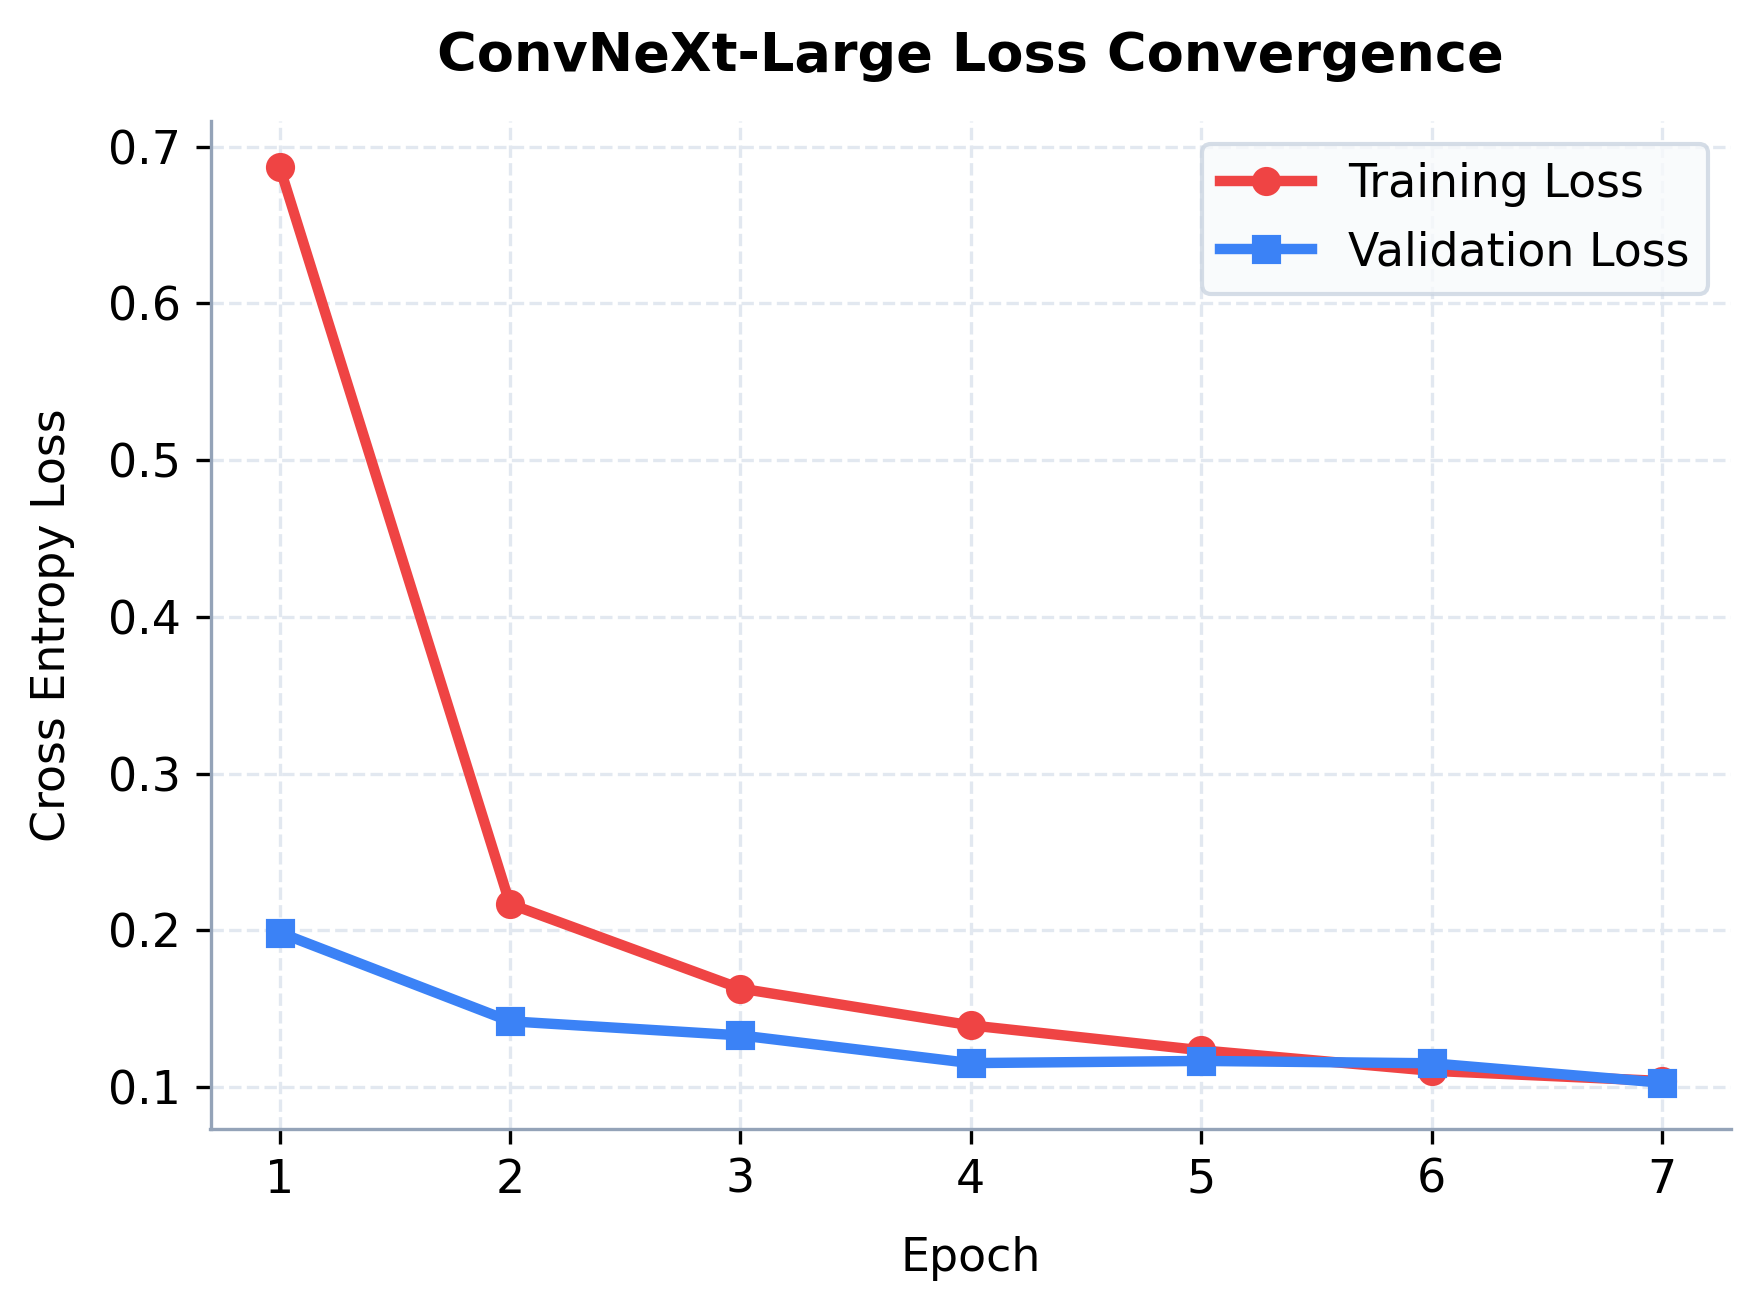
\includegraphics[width=0.6\textwidth]{loss_curve.png}
    \caption{Training and validation cross-entropy loss convergence over 7 training epochs for the cloud tier model.}
    \label{fig:loss_curve}
\end{figure}

\begin{figure}[htbp]
    \centering
    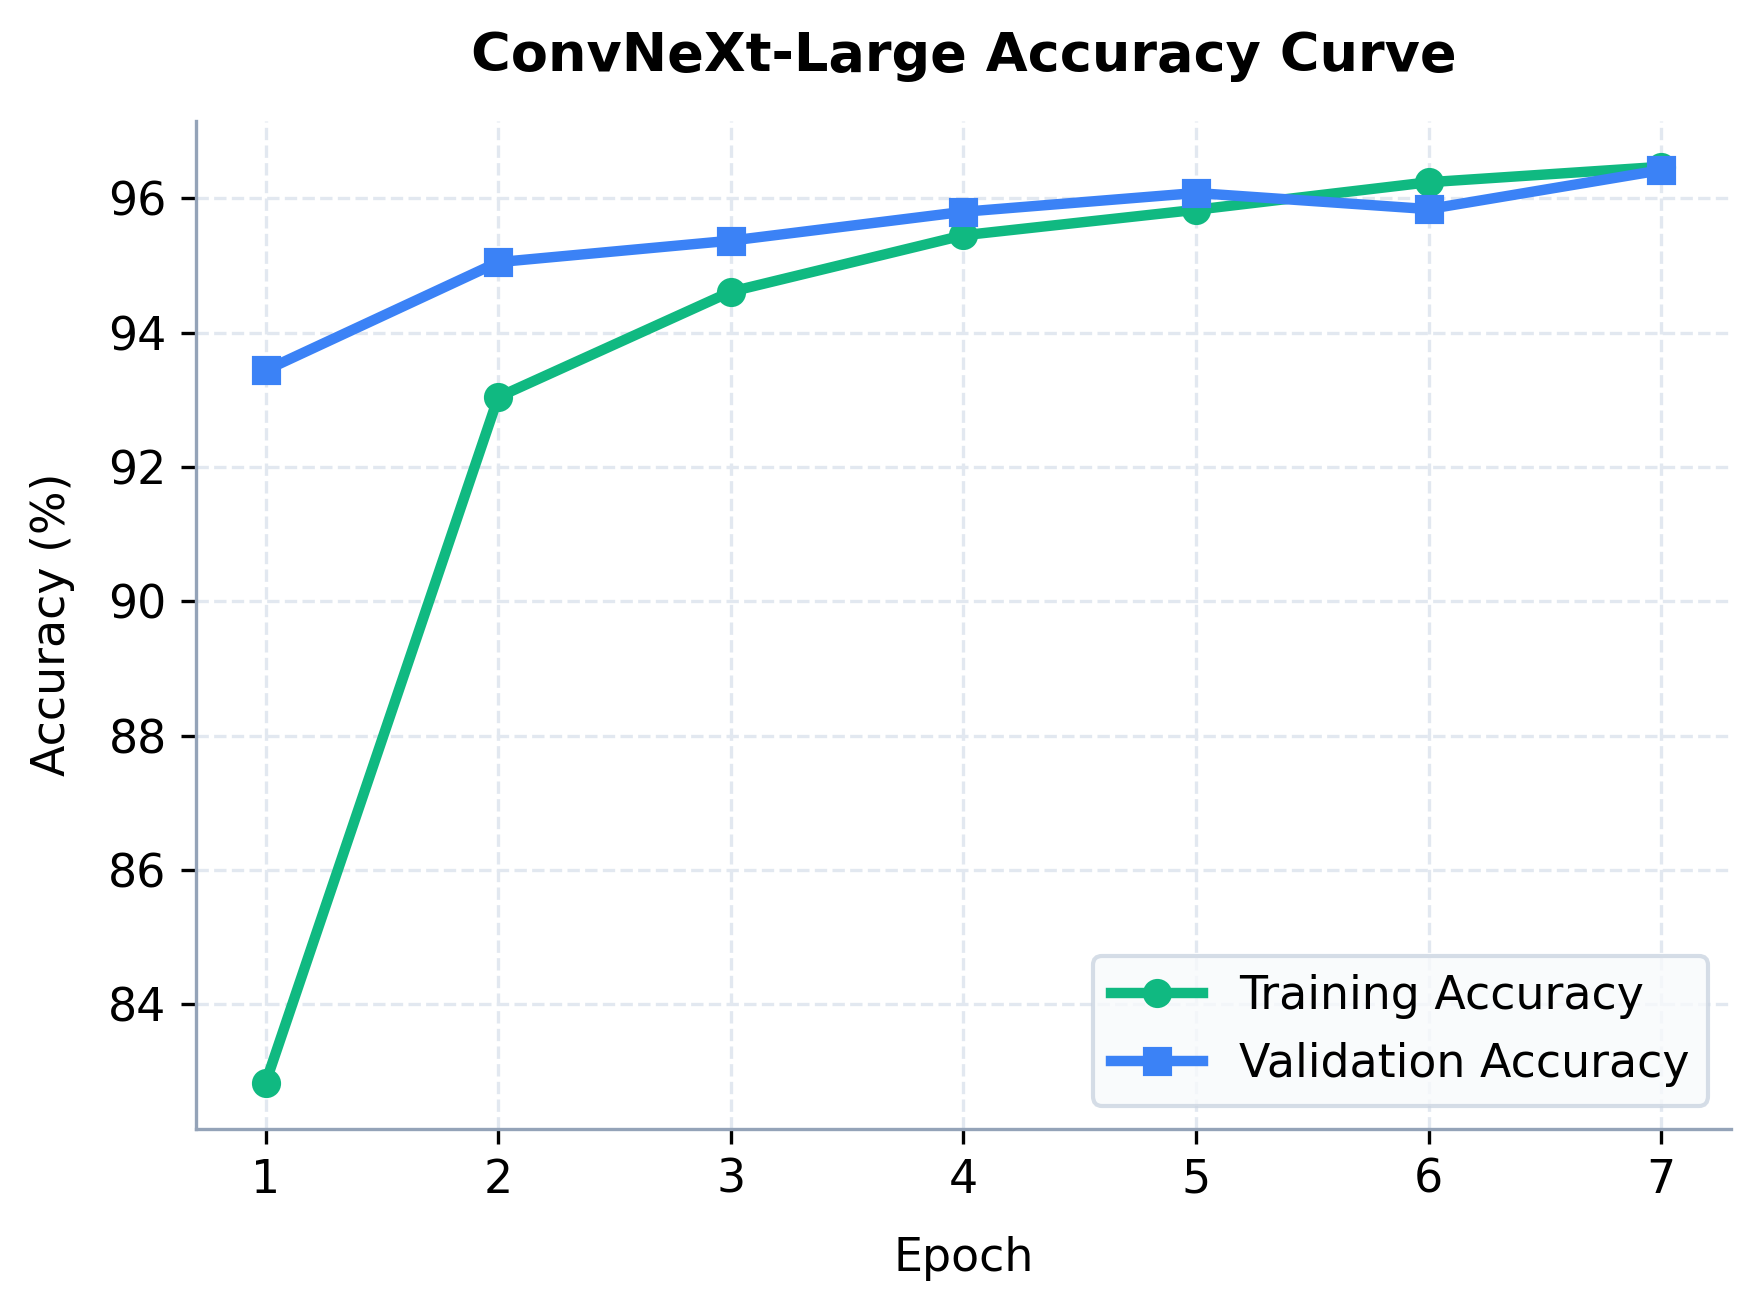
\includegraphics[width=0.6\textwidth]{accuracy_curve.png}
    \caption{Training and validation classification accuracy curves showing stable improvement up to 96.42\% accuracy.}
    \label{fig:accuracy_curve}
\end{figure}

\section{Experimental Results: Edge Model Convergence}
The lightweight edge model (\texttt{MobileNetV4-Conv-Medium} with Evidential Head and Domain Adaptation) was trained on the plant dataset over $10$ epochs. The multi-task loss is optimized using the AdamW optimizer with a learning rate $\eta = 10^{-3}$ and weight decay $10^{-3}$. All stages of the backbone are unfrozen to adapt from scratch to the 88 plant classes.

The training parameters and metrics extracted from the edge model logs are summarized in Table~\ref{tab:edge_metrics}.

\begin{table}[h]
\centering
\caption{Edge Model (\texttt{MobileNetV4-EDL}) Convergence Metrics}
\label{tab:edge_metrics}
\begin{tabular}{ccccccc}
\toprule
\textbf{Epoch} & \textbf{Train Cls Loss} & \textbf{Train Dom Loss} & \textbf{Train Acc (\%)} & \textbf{Val Loss} & \textbf{Val Accuracy (\%)} & \textbf{Val Vacuity ($u$)} \\
\midrule
1  & 2.0984 & 0.0245 & 67.60 & 1.5441 & 81.49 & 0.9606 \\
2  & 1.5398 & 0.0119 & 81.84 & 1.5426 & 82.20 & 0.9557 \\
3  & 1.4037 & 0.0110 & 85.19 & 1.4969 & 83.47 & 0.9433 \\
4  & 1.3306 & 0.0118 & 86.85 & 1.2157 & 88.87 & 0.8990 \\
5  & 1.2750 & 0.0122 & 87.91 & 1.2090 & 88.82 & 0.9011 \\
6  & 1.2260 & 0.0201 & 88.87 & 1.1313 & 90.27 & 0.8808 \\
7  & 1.1976 & 0.0199 & 89.49 & 1.0826 & 91.61 & 0.8664 \\
8  & 1.1430 & 0.0199 & 90.36 & 1.1093 & 90.55 & 0.8598 \\
9  & 1.1305 & 0.0212 & 90.40 & 0.9965 & \textbf{92.23} & \textbf{0.8219} \\
10 & 1.1171 & 0.0213 & \textbf{90.99} & 1.0341 & 91.97 & 0.8321 \\
\bottomrule
\end{tabular}
\end{table}

The loss convergence (including domain adversarial loss) and accuracy/vacuity dynamics are visualized in Fig.~\ref{fig:edge_loss_curve} and Fig.~\ref{fig:edge_accuracy_curve}, respectively. The validation accuracy achieved a peak of \textbf{92.23\%} at Epoch 9, with the average evidential uncertainty (vacuity) dropping to its lowest value of \textbf{0.8219}, signaling high classification certainty on the validation split. By Epoch 10, the classification loss converged to \textbf{1.1171} and training accuracy reached \textbf{90.99\%}, demonstrating stable joint optimization under domain adaptation and evidential constraints.

\begin{figure}[htbp]
    \centering
    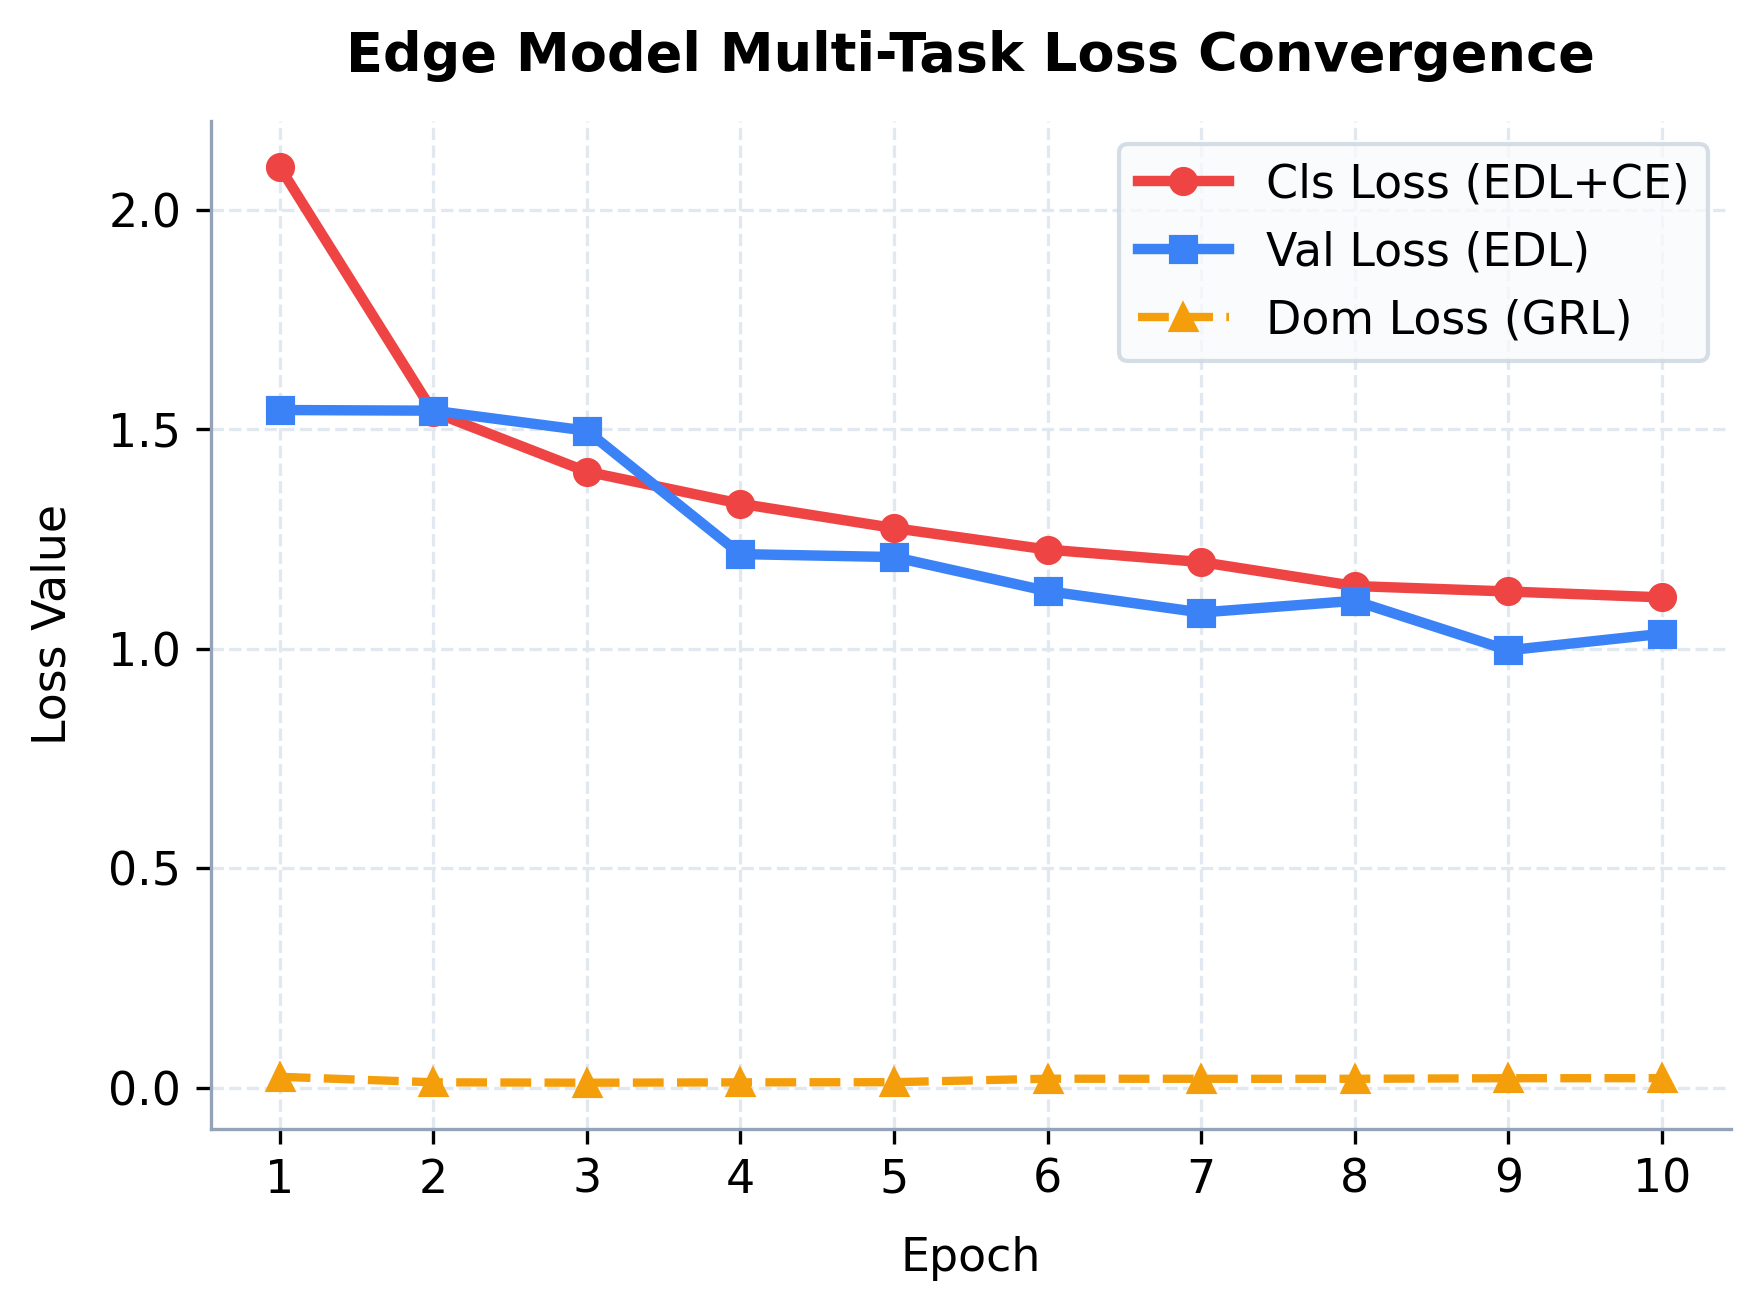
\includegraphics[width=0.6\textwidth]{edge_loss_curve.png}
    \caption{Multi-task loss convergence of the Edge model, showing the classification loss (EDL+CE), validation loss, and GRL domain adaptation loss.}
    \label{fig:edge_loss_curve}
\end{figure}

\begin{figure}[htbp]
    \centering
    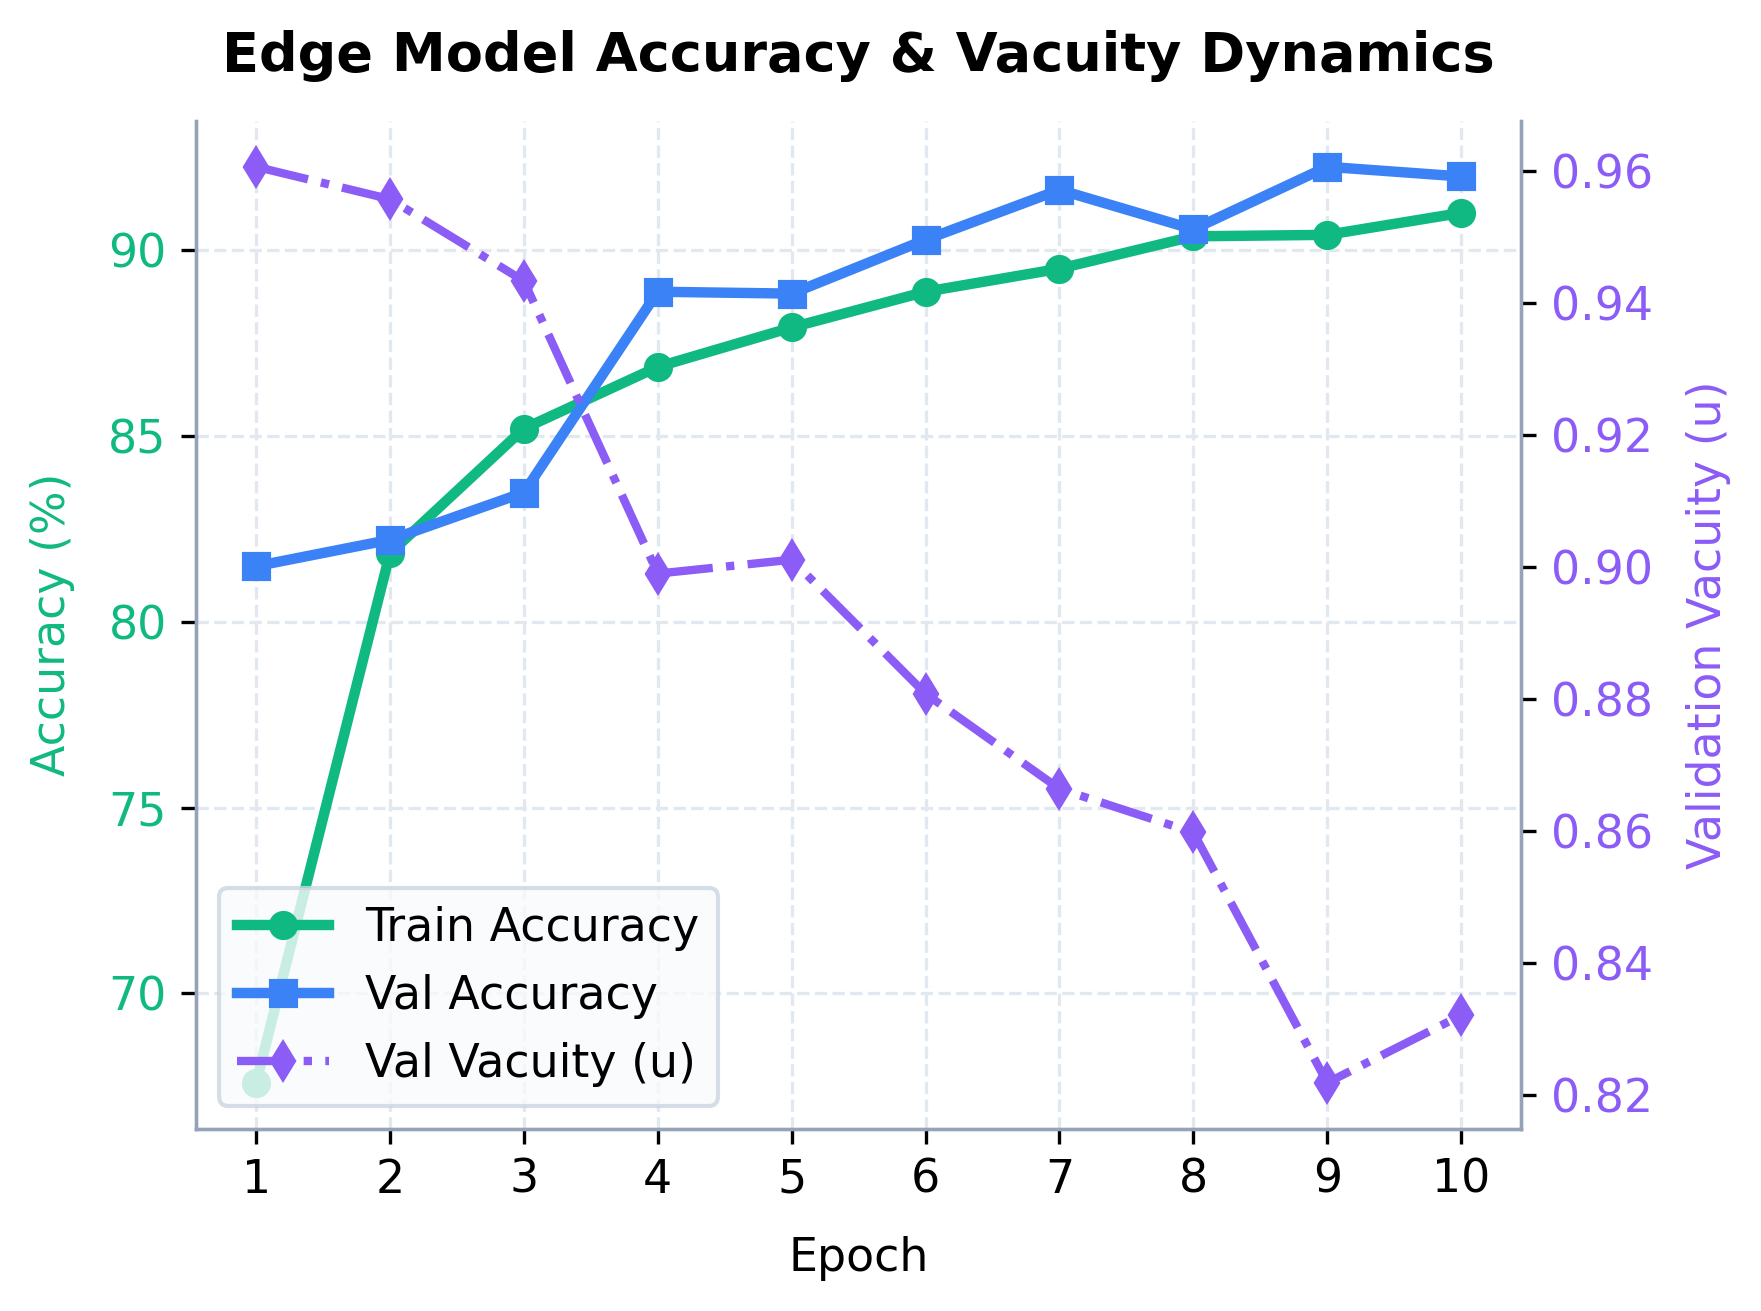
\includegraphics[width=0.6\textwidth]{edge_accuracy_curve.png}
    \caption{Edge model training and validation classification accuracy curves plotted alongside the validation average vacuity score ($u$).}
    \label{fig:edge_accuracy_curve}
\end{figure}

\end{document}
